\documentclass{beamer}
\usepackage[utf8]{inputenc}
\usepackage[croatian]{babel}
\usepackage{float}
\usepackage{amsmath}
\usepackage{graphicx} 
\usepackage{booktabs}
\mode<presentation> {
\usetheme{Madrid}
\usecolortheme{default}
\setbeamertemplate{navigation symbols}{} % To remove the navigation symbols from the bottom of all slides uncomment this line
}

\selectlanguage{croatian}
\author{Ivan Relić}

\title[Sveučilište u Zagrebu, FER]{Detekcija sigurnosnih atributa prometnica u snimkama} 


\begin{document}

\begin{frame}
\titlepage 
\end{frame}

\section{Uvod}

\begin{frame}
\frametitle{Uvod}
\begin{itemize}
\item iRAP -- međunarodna organizacija za inspekciju kvalitete cesta
\item ocjena kvalitete ceste na temelju sigurnosnih atributa (pripajanja, ograničenja brzine, osvjetljenje, broj traka, objekti pored ceste...)
\item zamjena procesa ručnog dodjeljivanja atributa strojnim
\item FTTS iRAP -- snimke engleskih autocesta s oznakama sigurnosnih atributa
 \end{itemize}

\end{frame}

\section{Zadatak}

\begin{frame}
 \frametitle{Zadatak}
 \begin{itemize}
  \item detektiranje atributa ``pripajanje trakova'' -- opasnost prilikom promjene traka
  \item binarna klasifikacija
  \item težina zadatka -- pojedinačne slike i sekvence
 \end{itemize}

 \begin{columns}
\begin{column}{0.5\textwidth}

\begin{figure}[H]
\centering
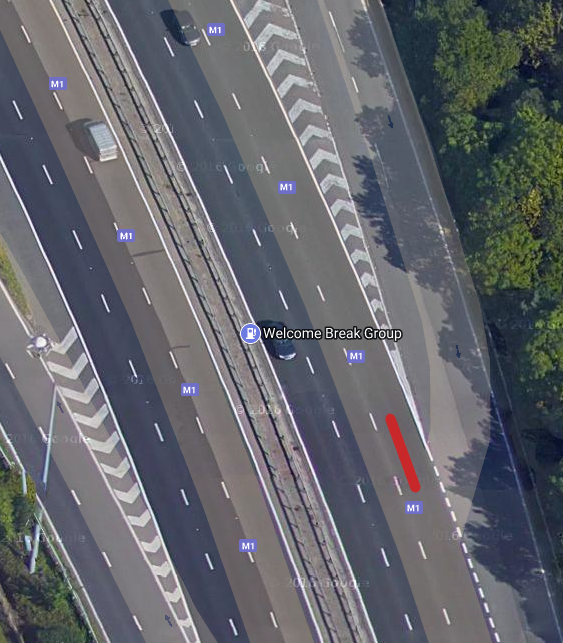
\includegraphics[scale=0.24]{images/sattelite.png}
\end{figure} 

\end{column}

\begin{column}{0.5\textwidth}
\begin{figure}[H]
\centering
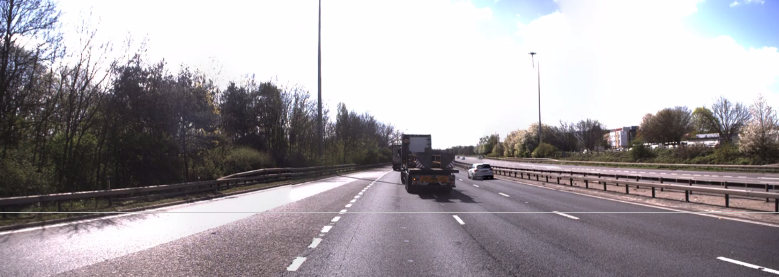
\includegraphics[scale=0.22]{images/car.png}
\end{figure} 

\begin{itemize}
 \item dva skupa podataka:
 \begin{itemize}
  \item skup podataka s diskriminativnim oznakama
  \item skup podataka s oznakama iz sustava FTTS iRAP
 \end{itemize}

\end{itemize}


\end{column}
\end{columns}
 
\end{frame}

\section{Skup podataka s diskriminativnim oznakama}
\begin{frame}

\frametitle{Skup podataka s diskriminativnim oznakama}

\begin{columns}
\begin{column}{0.6\textwidth}
\begin{figure}[H]
\centering
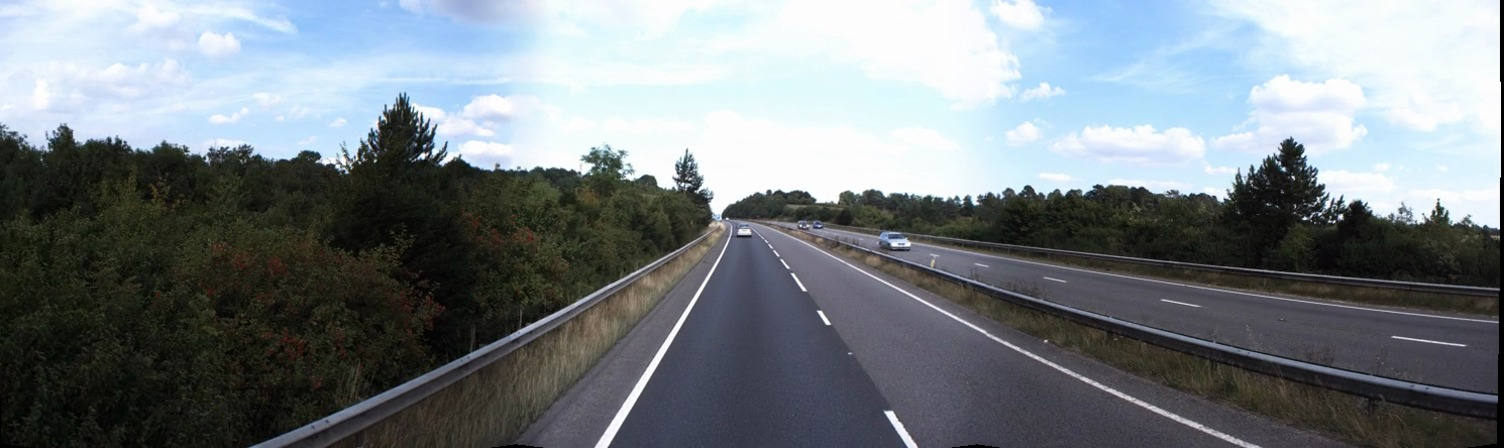
\includegraphics[scale=0.14]{images/discriminative_negative.jpg}
\end{figure} 

\begin{figure}[H]
\centering
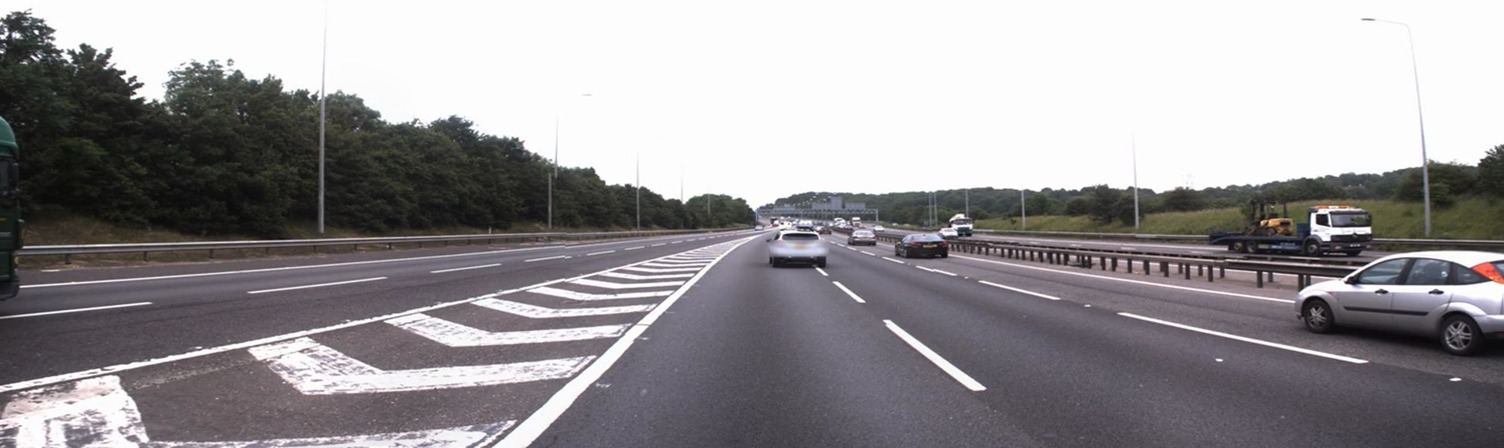
\includegraphics[scale=0.14]{images/discriminative_positive.jpg}
\end{figure} 
\end{column}
\begin{column}{0.4\textwidth}
\begin{itemize}
  \item raspodjela po podskupovima:
  \begin{itemize}
   \item učenje -- 1796 slika
   \item validacija -- 626 slika
   \item testiranje -- 594 slike
  \end{itemize}
  \item rezolucije:
  \begin{itemize}
   \item $700$x$280$
   \item $525$x$210$
   \item $350$x$140$
   \item $175$x$70$
  \end{itemize}

 \end{itemize}
\end{column}

\end{columns}
\end{frame}


\section{Skup podataka s oznakama iz sustava FTTS iRAP}
\begin{frame}

\frametitle{Skup podataka s oznakama iz sustava FTTS iRAP}

\begin{figure}[H]
\centering
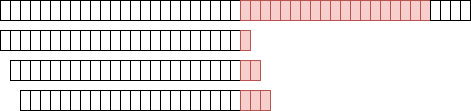
\includegraphics[scale=0.5]{images/sequence_making.png}
\end{figure} 

\begin{itemize}
\item generiran automatiziranim postupkom -- georeferencirane videosnimke, geolokacije pripajanja
\item svakoj slici pridružena geolokacija
 \item pojedinačne slike + sekvence duljine 25 slika
 \item pojedinačne slike rezolucije $700$x$280$
 \item sekvence slika rezolucije $350$x$140$
   \item raspodjela po podskupovima:
  \begin{itemize}
   \item učenje -- 7554 sekvenci
   \item validacija -- 1720 sekvenci
   \item testiranje -- 1642 sekvenci
  \end{itemize}
 \end{itemize}

\end{frame}

\section{Korištene arhitekture}
\begin{frame}
\frametitle{Korištene arhitekture}
 \begin{figure}[H]
\centering
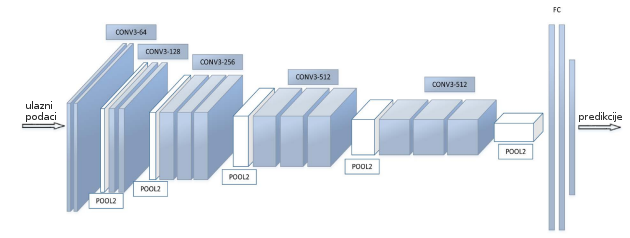
\includegraphics[scale=0.5]{images/vgg_architecture.png}
\end{figure} 
\begin{itemize}
 \item zasnovane na prednaučenoj arhitekturi VGG-16 namijenjenoj klasifikaciji slika 
 \item uklonjeni posljednji potpuno povezani slojevi
\end{itemize}
\end{frame}

\begin{frame}
\frametitle{Arhitektura za klasifikaciju pojedinačnih slika}
 \begin{figure}[H]
\centering
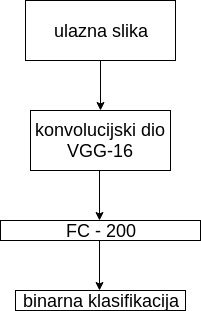
\includegraphics[scale=0.5]{images/single_image_architecture.png}
\end{figure} 
 \begin{itemize}
  \item eksperimenti na slikama s diskriminativnim oznakama i na pojedinačnim slikama s oznakama iz sustava FTTS iRAP
 \end{itemize}

\end{frame}

\begin{frame}
\frametitle{Arhitektura za klasifikaciju sekvenci korištenjem vremensko-prostornog sažimanja}

 \begin{figure}[H]
\centering
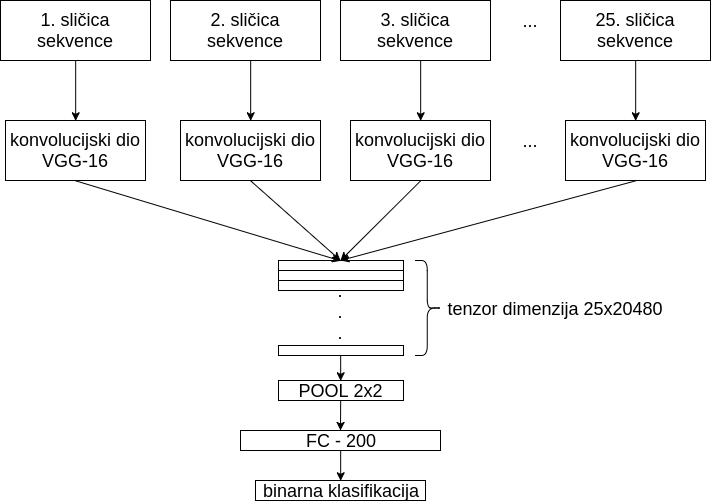
\includegraphics[scale=0.35]{images/sequence_pooling.png}
\end{figure} 

\end{frame}

\begin{frame}
\frametitle{Arhitektura za klasifikaciju sekvenci korištenjem LSTM ćelija}

 \begin{figure}[H]
\centering
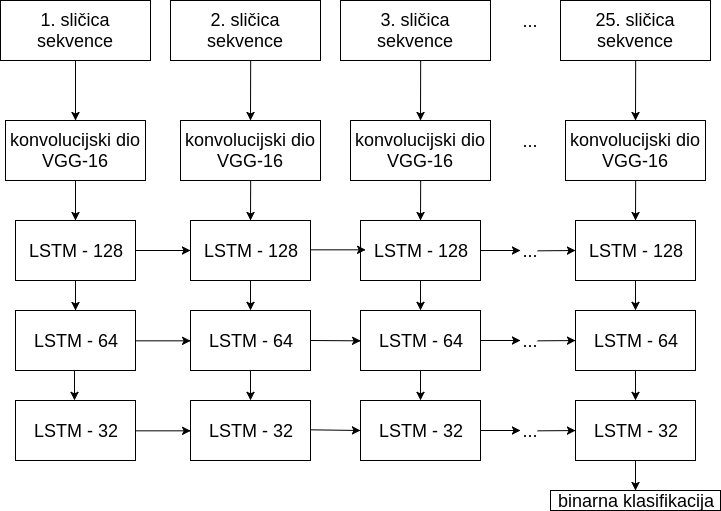
\includegraphics[scale=0.35]{images/sequence_lstm.png}
\end{figure} 

\end{frame}

\begin{frame}
\frametitle{Arhitektura za klasifikaciju sekvenci korištenjem vremenskog potpuno povezanog sloja}

 \begin{figure}[H]
\centering
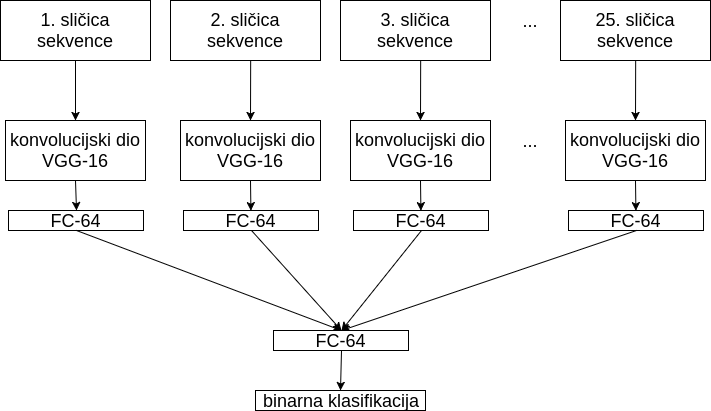
\includegraphics[scale=0.35]{images/sequence_temporal.png}
\end{figure} 

\end{frame}

\section{Rezultati}

\begin{frame}
 \frametitle{Učenje}
 \begin{itemize}
 \item nVidia GTX 1070 i GTX Titan
  \item 50 epoha -- 10 epoha ($5\cdot10^{-4}$, samo novo nadodani parametri) + 40 epoha ($1\cdot10^{-5}$, svi parametri)
  \item mini grupe veličina 5 ili 10, ovisno o memorijskoj zahtjevnosti
  \item učenje postupkom Adam, eksponencijalno smanjivanje stope učenja -- 0.96 u svakoj epohi
  \item svi parametri konvolucijskih i potpuno povezanih slojeva regularizirani L2 normom s faktorom regularizacije $5\cdot10^{-4}$
  \item normalizacija po mini grupama za sve potpuno povezane slojeve osim za binarnu klasifikaciju
  \item aktivacijske funkcije -- ReLU i softmax
  \item podskup za validaciju:
  \begin{itemize}
   \item rano zaustavljanje
   \item validacija praga
  \end{itemize}

 \end{itemize}

\end{frame}


\begin{frame}
 \frametitle{Rezultati na slikama s diskriminativnim oznakama}
 \begin{itemize}
  \item različite rezolucije ulaznih slika
  \item eksperiment proveden za pronalaženje najniže rezolucije na kojoj su performanse zadovoljavajuće
 \end{itemize}
 
 \begin{table}[H]
\centering
\caption{Rezultati na podskupu za testiranje}
\label{score:single_hand_test_resolutions}
\begin{tabular}{|c|c|c|c|c|}
\hline
rezolucija slika & točnost & preciznost & odziv & prosječna preciznost \\ \hline
700x280          &     0.93    &   0.88         &   1.0    &       0.99               \\ \hline
525x210          &    0.98     &    0.97        &   0.99    &       1.0               \\ \hline
350x140          &     0.98    &    0.96        &   0.99    &        0.99              \\ \hline
175x70           &    0.87     &    0.84        &   0.90    &      0.92                \\ \hline
\end{tabular}
\end{table}

\end{frame}


\begin{frame}
 \frametitle{Rezultati na pojedinačnim slikama s oznakama iz sustava FTTS iRAP}
 \begin{itemize}
  \item rezolucija ulaznih slika $700$x$280$
  \item učenje: 20.89 slika/sec, evaluacija: 25.59 slika/sec
 \end{itemize}
 
\begin{table}[H]
\centering
\caption{Rezultati}
\label{score:single_irap}
\begin{tabular}{c|c|c|c|c|}
\cline{2-5}
                                            & točnost & preciznost & odziv & prosječna preciznost \\ \hline
\multicolumn{1}{|c|}{učenje}     & 0.95       & 0.94        & 0.96     &           0.99           \\ \hline
\multicolumn{1}{|c|}{validacija} & 0.88       & 0.92        & 0.83     &            0.93          \\ \hline
\multicolumn{1}{|c|}{testiranje} & 0.83       & 0.87        & 0.77     &            0.91          \\ \hline
\end{tabular}
\end{table}

\begin{itemize}
 \item lošiji rezultati u odnosu na slike s diskriminativnim oznakama
\end{itemize}

\end{frame}

\begin{frame}
 \frametitle{Rezultati na sekvencama slika s oznakama iz sustava FTTS iRAP}
 \begin{itemize}
  \item rezolucija ulaznih slika $350$x$140$
  \item arhitektura koja koristi vremensko-prostorno sažimanje
    \item učenje: 3.93 sekvence/sec, evaluacija: 4.95 sekvenci/sec
 \end{itemize}
 
\begin{table}[H]
\centering
\caption{Rezultati}
\label{score:pooling}
\begin{tabular}{c|c|c|c|c|}
\cline{2-5}
                                            & točnost & preciznost & odziv & prosječna preciznost \\ \hline
\multicolumn{1}{|c|}{učenje}     & 0.91       & 0.96        & 0.85     &           0.97           \\ \hline
\multicolumn{1}{|c|}{validacija} & 0.89       & 0.96        & 0.82     &            0.95          \\ \hline
\multicolumn{1}{|c|}{testiranje} & 0.80       & 0.93        & 0.65     &            0.91          \\ \hline
\end{tabular}
\end{table}

\begin{itemize}
 \item nema poboljšanja u odnosu na pojedinačne slike
\end{itemize}

\end{frame}

\begin{frame}
 \frametitle{Rezultati na sekvencama slika s oznakama iz sustava FTTS iRAP}
 \begin{itemize}
  \item rezolucija ulaznih slika $350$x$140$
  \item arhitektura koja koristi LSTM slojeve
  \item učenje: 3.68 sekvenci/sec, evaluacija: 4.6 sekvenci/sec
 \end{itemize}
 
\begin{table}[H]
\centering
\caption{Rezultati}
\label{score:lstm}
\begin{tabular}{c|c|c|c|c|}
\cline{2-5}
                                            & točnost & preciznost & odziv & prosječna preciznost \\ \hline
\multicolumn{1}{|c|}{učenje}     & 0.98       & 0.98        & 0.99     &           0.99           \\ \hline
\multicolumn{1}{|c|}{validacija} & 0.90       & 0.94        & 0.85     &            0.94          \\ \hline
\multicolumn{1}{|c|}{testiranje} & 0.86       & 0.88        & 0.82     &            0.93          \\ \hline
\end{tabular}
\end{table}

\begin{itemize}
 \item poboljšanje u odnosu na pojedinačne slike
\end{itemize}


\end{frame}

\begin{frame}
 \frametitle{Rezultati na sekvencama slika s oznakama iz sustava FTTS iRAP}
 \begin{itemize}
  \item rezolucija ulaznih slika $350$x$140$
  \item arhitektura koja koristi vremenski potpuno povezani sloj
  \item učenje: 3.73 sekvence/sec, evaluacija: 4.81 sekvenci/sec
 \end{itemize}
 
\begin{table}[H]
\centering
\caption{Rezultati}
\label{score:temporal}
\begin{tabular}{c|c|c|c|c|}
\cline{2-5}
                                            & točnost & preciznost & odziv & prosječna preciznost \\ \hline
\multicolumn{1}{|c|}{učenje}     & 0.99       & 0.99        & 1.0     &           1.0           \\ \hline
\multicolumn{1}{|c|}{validacija} & 0.89       & 0.99        & 0.79     &            0.96          \\ \hline
\multicolumn{1}{|c|}{testiranje} & 0.86       & 0.96        & 0.74     &            0.94          \\ \hline
\end{tabular}
\end{table}

\begin{itemize}
 \item najveće poboljšanje u odnosu na pojedinačne slike
\end{itemize}


\end{frame}

\begin{frame}
 \frametitle{Analiza pogrešaka i detekcija krivih oznaka}
 \begin{itemize}
  \item evaluacija koristeći model koji koristi vremenski potpuno povezani sloj
  \item većina pogrešnih predikcija su lažni negativi (91\%)
  \item analiza geolokacija krivih predikcija -- atribut pripajanja pridružen drugom traku u 336/429 slučajeva (78\%)
  \item skup podataka kontaminiran krivim oznakama
 \end{itemize}
 
  \begin{figure}[H]
\centering
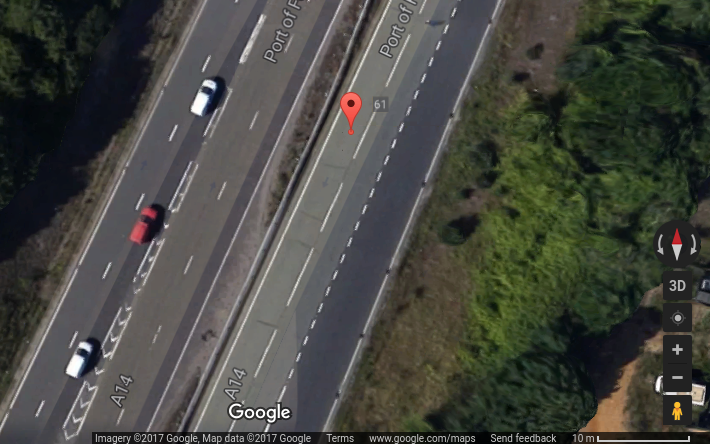
\includegraphics[scale=0.25]{images/wrong_lane_label.png}
\end{figure} 

\end{frame}

\section{Zaključak}

\begin{frame}
\frametitle{Zaključak}
 \begin{itemize}
  \item zadovoljavajuće performanse s obzirom na kontaminiranost skupa podataka
  \item koristeći geolokacije validirati oznake i generirati novi, pročišćeni skup podataka
  \item rjeđe uzorkovane, dulje sekvence slika
  \item modernije arhitekture
 \end{itemize}

\end{frame}

\begin{frame}
\Huge{\centerline{Hvala na pažnji!}}
\end{frame}

\end{document} 
